
\begin{quote}
\noindent {\em Generally, we are interested in multiphysics simulations---these
           combine a little bit of everything we discussed so far}
\end{quote}

\section{Integrating Multiphysics}

Method of lines vs.\ operator splitting

\section{Ex: diffusion-reaction}

Consider a diffusion-reaction equation:
\begin{equation}
\phi_t = \kappa \phi_{xx} = \frac{1}{\tau} R(\phi)
\end{equation}
This can be thought of as a simple model for a combustion flame, and
can propagate a front.  It is often the case that the reactions are
stiff, and require a smaller timestep then the diffusion part.  In
fact, we may want to use an implicit integration method designed for
stiff ODEs for the reaction part, but use a standard explicit method
for the diffusion part.  This requires operator splitting.

We can use Strang splitting \cite{strang} to make the integration
second-order accurate overall:
\begin{equation}
\phi^{n+1} = R_{\Delta t/2} D_{\Delta t} R_{\Delta t/2} \phi^n
\end{equation}
where $R_{\Delta t/2}$ represents reacting for a step of $\Delta t/2$
and $D_{\Delta t}$ represents diffusing for a step of $\Delta t$.  In
each case, these operators act as if the other were not present, but
they see the effect of the previous operation on the input $\phi$.  

No explict source terms describing one process appear in the other
process' update.  The procedure for updating appears as:
\begin{enumerate}
\item {\em Evolve reaction ODE system for $\Delta t/2$}
   %
   \begin{equation}
   \frac{d\phi^\star}{dt} = \frac{1}{\tau} R(\phi^\star), \qquad 
   \phi^\star(0) = \phi^n
   \end{equation}

\item {\em Solve the diffusion equation for $\Delta t$ with an
           implicit Crank-Nicolson discretization}
   %
   \begin{equation}
   \frac{\phi^{\star\star} - \phi^\star}{\Delta t} =
      \frac{1}{2} (D(\phi^\star) + D(\phi^{\star\star}))
   \end{equation}

\item {\em Evolve reaction ODE system for $\Delta t/2$}
   %
   \begin{equation}
   \frac{d\phi^{n+1}}{dt} = \frac{1}{\tau} R(\phi^{n+1}), \qquad 
   \phi^{n+1}(0) = \phi^{\star\star}
   \end{equation}

\end{enumerate}

Figure~\ref{fig:diffreact} shows the solution to our diffusion-reaction
equation with 256 zones, $\kappa = 0.1$, $\tau = 1.0$ at several times.

\begin{figure}[t]
\centering
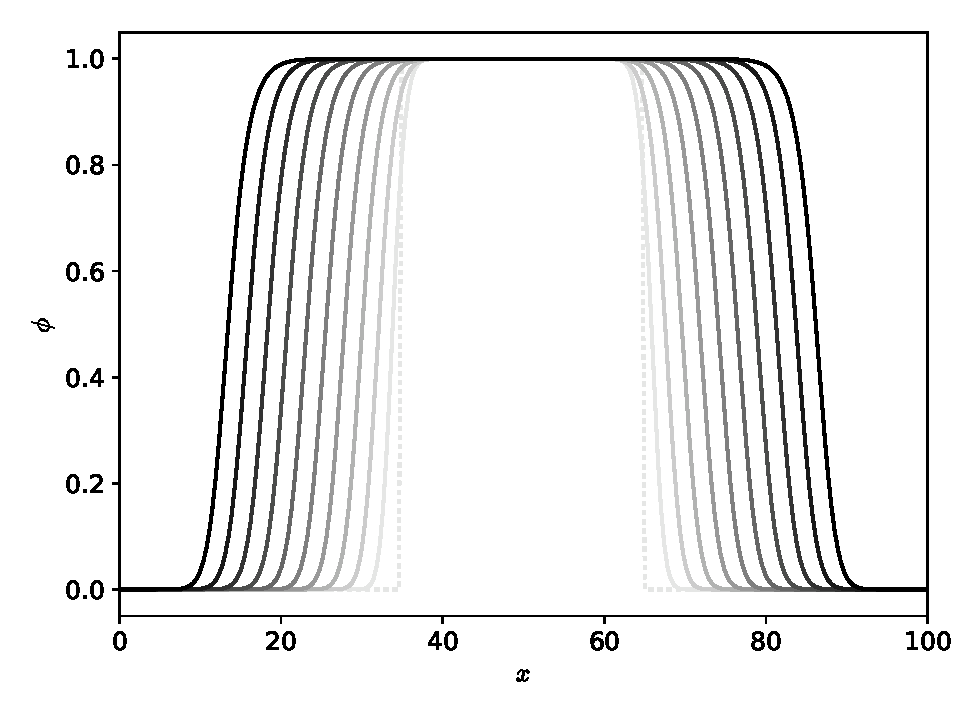
\includegraphics[width=5.0in]{flame_seq}
\caption[Solution to the diffusion-reaction equation]
  {\label{fig:diffreact} Solution to the diffusion-reaction equation
   with 256 zones, and $\kappa = 0.1$, $\tau = 1.0$.  The lines shown
   are spaced 8.0 time-units apart.  We see the initial smoothed tophat
   profile giving rise to a traveling front. \\
   \hydroexdoit{\href{https://github.com/zingale/hydro_examples/blob/master/multiphysics/diffusion-reaction.py}{diffusion-reaction.py}}
   }
\end{figure}


\begin{exercise}[Diffusion-reaction system]
 Consider a simple reaction source
 \begin{equation}
 R(\phi) = \frac{1}{4} \phi (1 - \phi)
 \end{equation}
 This is called a KPP reaction source.
 Here $\phi$ can be thought of as a progress variable that varies
 between pure ash ($\phi = 0$) and pure fuel ($\phi = 1$).

 Solve the system with this source.  Note that you should begin with
 some smooth initial conditions---if they are too sharp than the 
 C-N discretization will cause jagged features to appear.  
 The solution in this case is a wave with speed $S = \sqrt{\kappa/\tau}$
 and thickness $\delta = \sqrt{\kappa \tau}$ (see \cite{vladimirova2006} for
 some details of this system).
\end{exercise}


\section{Ex: advection-diffusion}

The viscous Burgers' equation appears as:
\begin{equation}
u_t + u u_x = \epsilon u_{xx}
\end{equation}
This admits shocks and rarefactions just like the inviscid form, but now
the viscosity can act to smooth out the shock---instead of being
infinitely thin, it will have a physical width.

As we saw earlier, there are efficient, accurate methods for handling
the explicit parts explicitly, but for diffusion, we often want to 
solve it implicitly.  We can split the solution up, but couple the 
two processes together to make a method that is overall second-order
accurate in time.  We write our equation as:
\begin{equation}
u_t + A(u) = D(u)
\end{equation}
with $A(u) = [\frac{1}{2} u^2]_x$ and $D(u) = eu_{xx}$.  Then our update 
appears in two steps.
\begin{enumerate}
\item {\em Find the advective update over the timestep}:
   We use an approximation of the diffusion term at time-level $n$, $D(u^n)$
   as a source in the construction of the interface states for the 
   advective part.  Once the interface states, $u_{i+1/2}^{n+1/2}$ are
   known, we construct the advective update term as:
   \begin{equation}
   A_i^{n+1/2} = 
     \frac{\left [ \frac{1}{2} \left (u_{i+1/2}^{n+1/2}\right)^2\right ] -
           \left [ \frac{1}{2} \left (u_{i-1/2}^{n+1/2}\right)^2\right ]}
          {\Delta x}
    \end{equation}

\item {\em Solve the diffusion equation with the advective source}:
    We use a Crank-Nicolson discretization of the diffusion part of 
    our equation, with the advective update term appearing as a source.
    \begin{equation}
    \frac{u^{n+1} - u^n}{\Delta t} = 
        \frac{1}{2}D(u^n) + \frac{1}{2}D(u^{n+1}) - A^{n+1/2}
    \end{equation}
    
    This is a linear system that can be solved as a tridiagonal matrix
    or with multigrid.  The result of this step is that $u^{n+1}$ is
    updated with both the advection and diffusion terms.

\end{enumerate}

Because the diffusion is done implicitly, the timestep constraint (for
stability) for this solve is due to the advective portion only.

\begin{figure}[t]
\centering
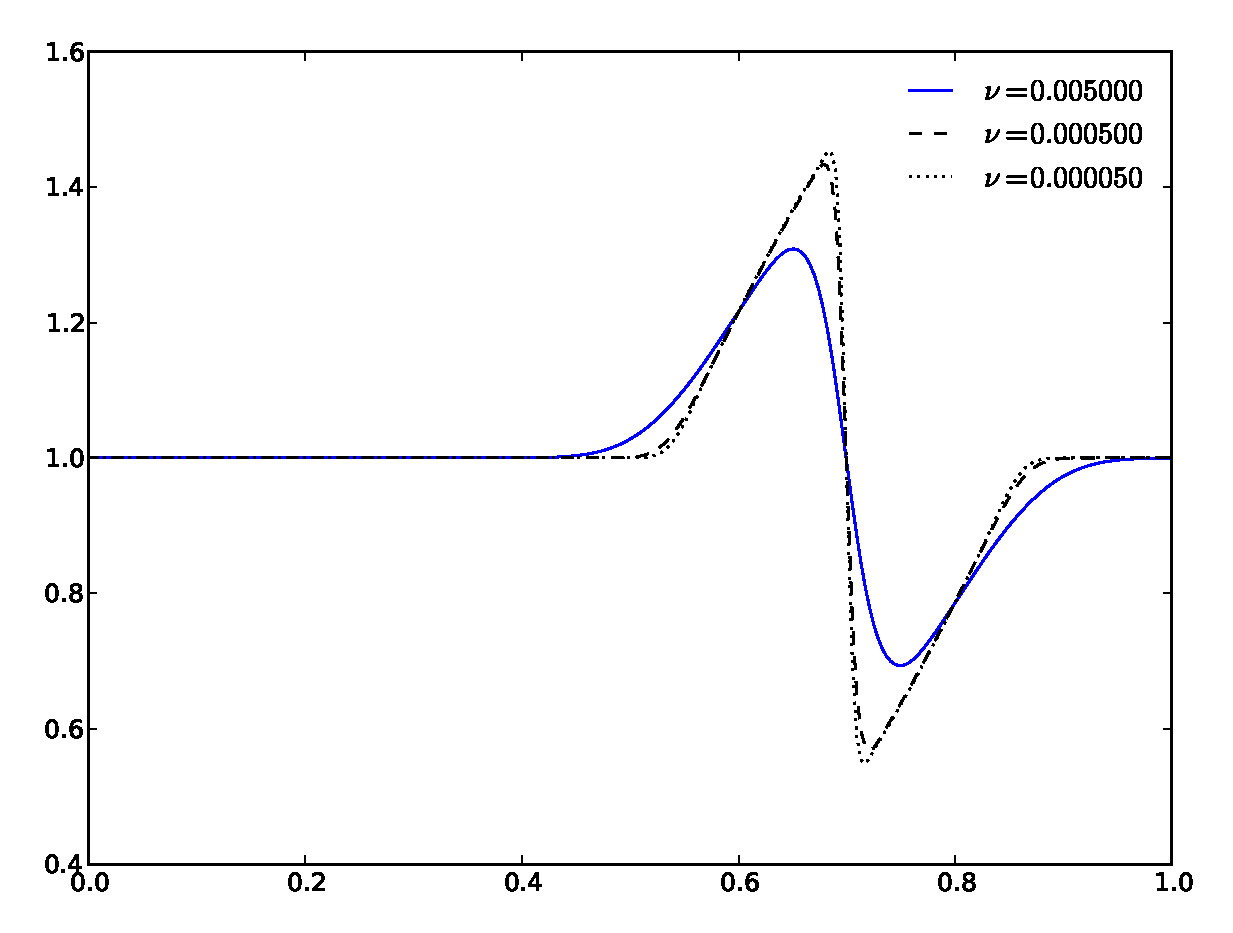
\includegraphics[width=5in]{burgervisc}
\caption[Viscous Burgers' equation solution.]
  {\label{fig:viscburger} Solution to the viscous Burgers' equation
  with a variety of different viscosities.  The initial conditions was
  a single wavelength of a sine wave for $x \in [1/3,2/3]$, and $u = 1$
  otherwise. \\
  \hydroexdoit{\href{https://github.com/zingale/hydro_examples/blob/master/multiphysics/burgersvisc.py}{burgersvisc.py}}}
\end{figure}

For step 1, the addition of the explicit diffusion source requires
a small change to the method we used to predict the interface states.

\begin{eqnarray}
u^{n+1}_{i+1/2,L} &=& u^n_i + \frac{\Delta x}{2} \frac{\partial u}{\partial x}
                        + \frac{\Delta t}{2} \frac{\partial u}{\partial t} + \ldots \\
                &=& u^n_i + \frac{\Delta x}{2} \frac{\partial u}{\partial x}
                        + \frac{\Delta t}{2} \left (-u_i \frac{\partial u}{\partial x} + D(u^n_i) \right ) + \ldots \\
                &=& u^n_i + \frac{\Delta x}{2} \left ( 1 - \frac{\Delta t}{\Delta x}u_i \right ) \frac{\partial u}{\partial x} + {\color{red} \frac{\Delta t}{2} D(u^n) } + \ldots
\end{eqnarray}
here the source term (shown in red) incorporates the effects of the
diffusion on the prediction of the states for advection.  This entered
into our states when we replaced $\partial u/\partial t$ with our PDE
equation.  The spatial derivative, $\partial u/\partial x$ is replaced
by a monotonized difference, and the method then proceeds as with the
regular Burgers' equation.  The Riemann problem is unchanged from the
inviscid case.

Figure~\ref{fig:viscburger} shows the solution of the viscous Burgers'
equation for shock initial conditions with different amounts of
viscosity.  Notice that the effect of the viscosity is to smooth the
shock profile, but the shock position itself agrees between the cases.


